% Section 5 --- Results. Figures are built by scripts/make_figures.py from the
% CSVs in results/; every number here is reproducible from those two files.
\section{Results}
\label{sec:results}

\subsection{The probes read truth where it matters}

Gate~A asks whether a probe beats the model's own stated confidence on the half
of items the model is most confident about. On TruthfulQA, where $42\%$ of
confident items are answered wrongly, \emph{every} model passes: the probe adds
between $0.05$ and $0.35$ AUROC over confidence. On the remaining datasets the
models are usually right when confident, confidence is therefore already a good
predictor, and the probe's advantage is smaller and sometimes absent. The
instrument works where there is work for it to do, and TruthfulQA is accordingly
where the oversight questions below are sharpest.

The unsupervised probe does not survive this test. CCS reads truth on curated
factual statements at $0.99$ AUROC and fails on adversarial misconceptions,
scoring below the confidence baseline on the confident slice --- the failure mode
\citet{farquhar2024challenges} predict, reproduced. All results below therefore
use a supervised probe, and the oversight claim is correspondingly ``fit once,
deploy without labels'' rather than label-free.

\subsection{False agreement, and where it sits inside its bound}

\begin{figure}[t]
\centering
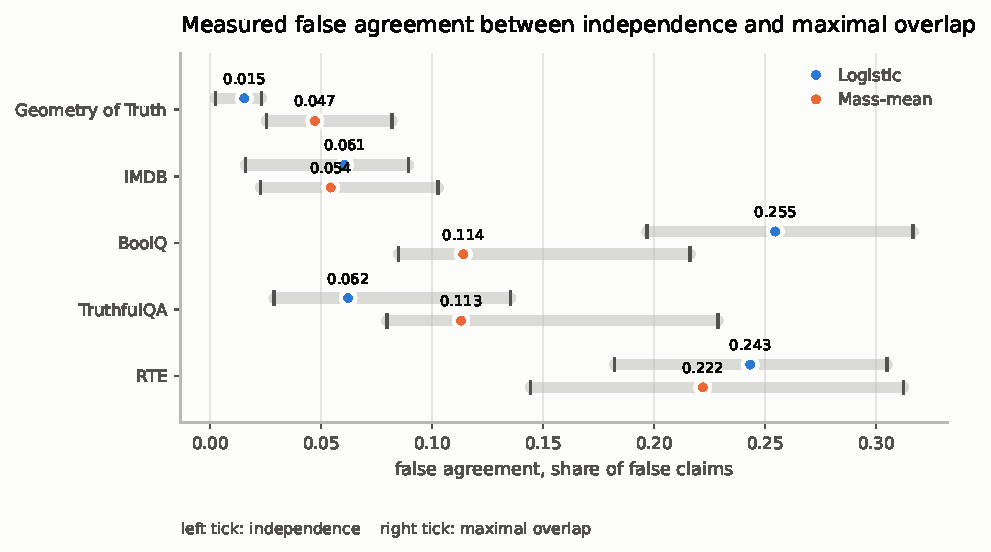
\includegraphics[width=\textwidth]{figures/fig1_bound}
\caption{False agreement against the interval the marginals permit. The track
runs from the rate two probes would hit by coincidence alone ($p_1p_2$) to the
ceiling set by the more accurate probe's own error rate ($\min(p_1,p_2)$);
the dot is what we measure, averaged over all pairs. Errors are far from
independent everywhere, and on Geometry of Truth and RTE they sit nearly half way
to the ceiling.}
\label{fig:bound}
\end{figure}

Figure~\ref{fig:bound} places the measured rate inside the interval
Section~\ref{sec:theory} derives. False agreement runs from $4.3\%$ of false
claims on Geometry of Truth to $22.4\%$ on RTE, with TruthfulQA at $14.1\%$. In
every dataset it sits well above the coincidence rate: the two probes' errors are
positively correlated in $83\%$ of the $228$ pair--dataset cells we measure, and
the pattern is not driven by a few outliers.

\paragraph{Family diversity does not reduce it.}
The obvious remedy fails, and the decomposition says why. Drawing the two models
from different families does lower the error correlation --- $\rho/\rho_{\max}$
falls from $0.409$ within a family to $0.291$ across --- but those pairs carry
higher individual error rates, and the two terms of the identity very nearly
cancel: false agreement is $12.9\%$ within families and $12.3\%$ across, a
difference of six tenths of a percentage point. What \emph{does} improve is
coverage of the overseen model's errors, from $0.423$ to $0.527$, because a less
correlated checker disagrees more often. Diversity buys disagreement, not a
smaller blind spot.

\subsection{What transport costs}

\begin{figure}[t]
\centering
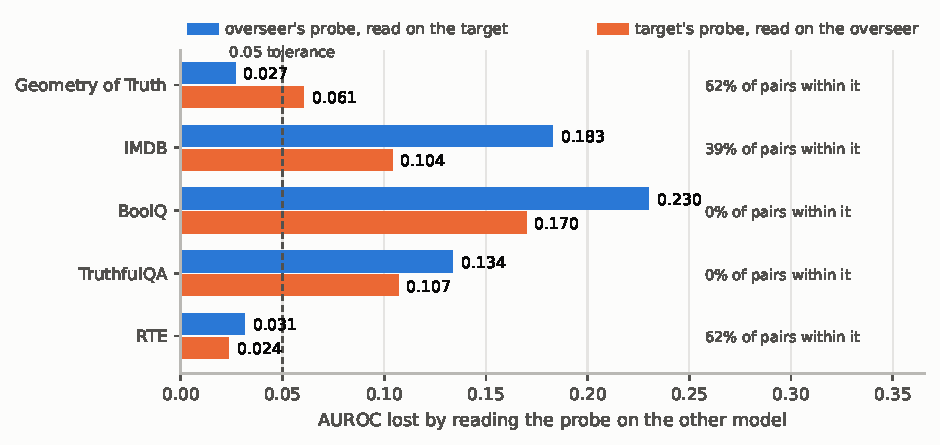
\includegraphics[width=\textwidth]{figures/fig2_transport}
\caption{AUROC a probe gives up when read on the other model through the
alignment map, by dataset and direction, with the share of pairs staying inside a
$0.05$ tolerance. Transport is close to free on curated factual statements and
fails on every BoolQ pair.}
\label{fig:transport}
\end{figure}

Transport is not a single fact about a pair of models; it is a fact about a pair
\emph{and} a dataset (Figure~\ref{fig:transport}). On Geometry of Truth a probe
read on the other model through the map loses $0.027$ AUROC and $62\%$ of pairs
stay within tolerance; on BoolQ it loses $0.23$ and \emph{no} pair does. The
asymmetry \citet{gorbett2026ventriloquist} report also appears here: averaged
over all cells, reading the larger model's probe on the smaller costs less than
the reverse ($0.094$ against $0.115$).

Representational similarity predicts this only loosely. CKA correlates with
transfer loss at $-0.51$ against the worse of the two directions, and the two
come apart in individual cells --- one pair sits at CKA $0.49$ with a transported
probe losing $0.004$. A probe needs one direction to survive where CKA grades all
of them.

\subsection{Is the blind spot detectable?}

\begin{figure}[t]
\centering
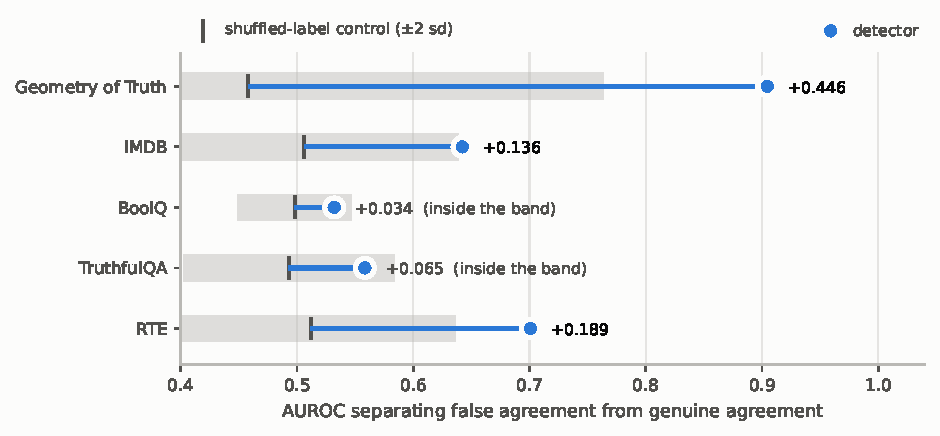
\includegraphics[width=\textwidth]{figures/fig3_detect}
\caption{Leave-one-dataset-out: probes, map and direction are fitted on four
datasets and deployed on a fifth none of them has seen. The bar is the
permutation control's own noise ($\pm 2$ sd); a detector inside it has not been
shown to work. The signature transfers decisively to curated factual statements
and barely at all to the two datasets where false agreement is most common.}
\label{fig:detect}
\end{figure}

If false agreement is made of shared error, shared error might leave a signature.
Figure~\ref{fig:detect} tests this in the hardest honest way: everything is
fitted on four datasets and deployed on a fifth, and the comparison is against
the same procedure run on shuffled labels.

The result is a split. On Geometry of Truth the direction separates false from
genuine agreement at $0.904$ AUROC against a $0.456$ control, a margin of
$+0.448$. On TruthfulQA and BoolQ the margins are $+0.065$ and $+0.034$, inside
or barely outside the control's own spread. The detector works where false
agreement is rare and templated, and not where it is common --- which is the
opposite of where an operator would want it. This is the representation-level
counterpart of \citet{afrin2026ensembles}, who prove the common-mode component of
evaluator error is not identifiable from the judges' own scores.

\subsection{What an operator gets}

\begin{figure}[t]
\centering
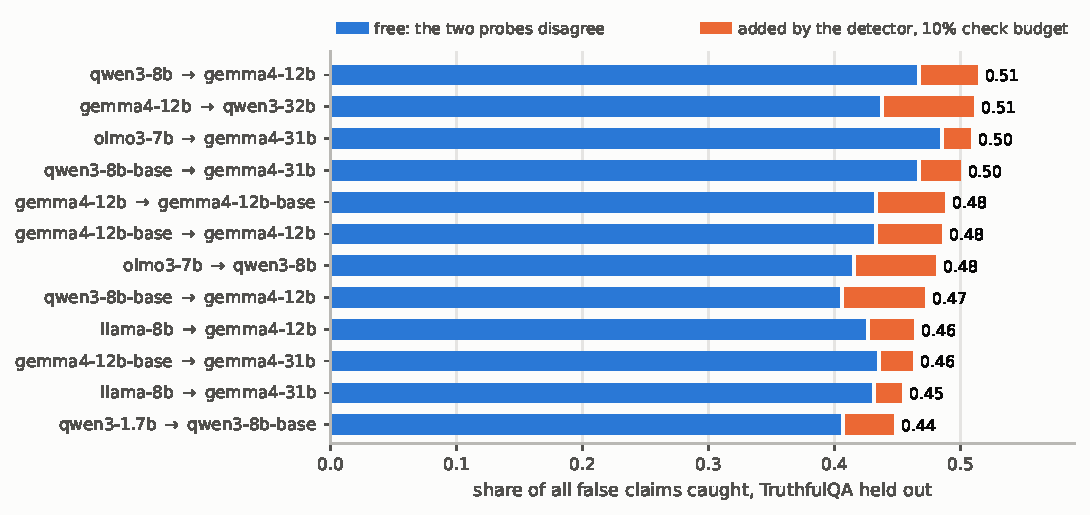
\includegraphics[width=\textwidth]{figures/fig4_pairs}
\caption{The twelve best pairs on TruthfulQA, by share of all false claims
caught. The blue segment is free --- the two probes disagree and the item is
routed --- and the orange segment is what the detector adds when a further
$10\%$ of agreeing items are checked. Across all pairs the free component
dominates.}
\label{fig:pairs}
\end{figure}

Putting the pieces together as a deployment (Figure~\ref{fig:pairs}): two probes
read a claim, disagreement routes it for an expensive check at no modelling cost,
and a budget of further checks is spent on the agreeing items the detector ranks
highest. On TruthfulQA the best pairs reach $0.51$ of all false claims caught at a
$10\%$ budget, against a mean of $0.39$, and almost all of that is the free
component: disagreement alone catches $0.336$.

The best pairs are instructive. \texttt{qwen3-8b}$\rightarrow$\texttt{gemma4-12b}
and \texttt{gemma4-12b}$\rightarrow$\texttt{qwen3-32b} both reach $0.51$, and
both are cross-family --- consistent with diversity buying disagreement rather
than a smaller blind spot. But cross-family and same-family pairs end up at
$0.393$ and $0.384$ on average, so the advantage is small once the detector's
contribution is included.

Two numbers bound the practical claim. Agreement between two models' internal
readouts catches roughly half of the overseen model's errors
($0.42$--$0.53$ depending on pairing). And when these two models agree that a
TruthfulQA claim is true, it is false $43\%$ of the time, so on confound-rich data
their agreement is close to uninformative on its own.
